\documentclass[11pt]{article}
\usepackage[margin=1in,letterpaper]{geometry}
\usepackage{amssymb,amsmath,amsthm,fancyhdr,supertabular,longtable,hhline}
\usepackage{colortbl}
\usepackage{import, multicol,boxedminipage}
\usepackage{graphicx}
\usepackage[colorlinks, hyperindex, plainpages=false, linkcolor=blue, urlcolor=blue, pdfpagelabels]{hyperref}
\usepackage[all]{hypcap}
\definecolor{ResultColor}{gray}{0.9}
\theoremstyle{definition}  % this prevents the text in definitions, theorems, and corollaries from being italicized
\newtheorem{defn}{\bf Definition}
\newtheorem{thm}{\bf Theorem}
\newtheorem{cor}[thm]{\bf Corollary}
\newtheorem{eqn}{\bf Equation}
\newtheorem{ex}{\bf Example}
\newtheorem{fig}{\bf Figure}
\setlength{\parindent}{0in}
\newcommand{\bbm}{\begin{boxedminipage}{6.41in}}
\newcommand{\ebm}{\end{boxedminipage}}
\usepackage{array}
\setlength{\extrarowheight}{2pt}
\allowdisplaybreaks[2]
\usepackage{cancel}
\usepackage{sectsty}
\usepackage{textcomp}
\usepackage{multirow}
\usepackage[sfdefault,lf]{carlito}
	%% The 'lf' option for lining figures
	%% The 'sfdefault' option to make the base font sans serif
	%\usepackage[T1]{fontenc}
	\renewcommand*\oldstylenums[1]{\carlitoOsF #1}
\usepackage[nottoc]{tocbibind}
\allsectionsfont{\mdseries \scshape}
\makeatletter
\renewcommand\l@section{\@dottedtocline{1}{1.5em}{3em}}
\renewcommand\l@subsection{\@dottedtocline{2}{4.5em}{3.5em}}
\makeatother
\pagestyle{fancy}
\newcounter{HW}
\newcounter{HWindent}

\title{Review \#1: Set Theory}
\author{Carl Stitz and Jeff Zeager\\
Edited by Sean Fitzpatrick}

\begin{document}
\maketitle


\renewcommand{\headrulewidth}{0pt}
\renewcommand{\headheight}{14pt}
\lhead[\fancyplain{}{\sc\thepage}]%
      {\fancyplain{}{\sc \nouppercase{\rightmark}}}
\rhead[\fancyplain{}{\sc \nouppercase{\leftmark}}]%
      {\fancyplain{}{\sc\thepage}}
\cfoot{}


\medskip

\colorbox{ResultColor}{\bbm

\begin{defn} \label{setdef}

A \textbf{set}\index{set ! definition of} is a well-defined collection of objects which are called the `elements' of the set.  Here, `well-defined' means that it is possible to determine if something belongs to the collection or not, without prejudice. 

\end{defn}

\ebm}

\medskip

The collection of letters that make up the word ``pronghorns'' is well-defined and is a set, but the collection of the worst Math teachers in the world is \textbf{not} well-defined\footnote{One thing that student evaluations teach us is that any given Mathematics instructor can be simultaneously the best and worst teacher ever, depending on who is completing the evaluation.} and and therefore is \textbf{not} a set.\footnote{For a more thought-provoking example, consider the collection of all things that do not contain themselves - this leads to the famous \href{http://en.wikipedia.org/wiki/Russell's_paradox}{\underline{Russell's Paradox}}.}  In general, there are three ways to describe sets and those methods are listed below.


\medskip

\phantomsection \label{waystodescribesets}

\colorbox{ResultColor}{\bbm

\centerline{\textbf{Ways to Describe Sets}}

\begin{enumerate}

\item \textbf{The Verbal Method:} Use a sentence to define the set.\index{set ! verbal description}

\item \textbf{The Roster Method:}  Begin with a left brace `$\{$', list each element of the set \textit{only once} and then end with a right brace `$\}$'.\index{set ! roster method}

\item \textbf{The Set-Builder Method:} A combination of the verbal and roster methods using a ``dummy variable'' such as $x$.\index{set ! set-builder notation}\index{set-builder notation}

\end{enumerate}

\ebm}

\medskip

For example, let $S$ be the set described \textit{verbally} as the set of letters that make up the word ``pronghorns''.  A  \textbf{roster} description of $S$ is $\left\{ p, r, o, n, g, h, s \right\}$. Note that we listed  the letters o, r, and  n only once, even though they appear twice in the word ``pronghorns''.  Also, the \textit{order} of the elements doesn't matter, so $\left\{ o, n, r, p, h, s, g \right\}$ is also a roster description of $S$.  Moving right along,  a \textbf{set-builder} description of $S$ is: $\{ x \, | \, \mbox{$x$ is a letter in the word ``pronghorns''}\}$.  The way to read this is `The set of elements $x$ \underline{such that} $x$ is a letter in the word ``pronghorns''.'   In each of the above cases, we may use the familiar equals sign `$=$' and write  $S = \left\{ p, r, o, n, g, h, s \right\}$ or $S = \{ x \, | \, \mbox{$x$ is a letter in the word ``pronghorns''}\}$.  

\smallskip

Notice that  $r$ is in $S$ but many other letters, such as $q$, are not in $S$.  We express these ideas of set inclusion and exclusion mathematically using the symbols $r \in S$ (read `$r$ \underline{is in} $S$') and $q \notin S$ (read `$q$ \underline{is not in} $S$').  More precisely, we have the following.

\medskip

\colorbox{ResultColor}{\bbm

\begin{defn} \label{notationforsetinclusion}  Let $A$ be a set.

\begin{itemize}

\item If $x$ is an element of $A$ then we write $x \in A$\index{set ! inclusion}\index{$\in$} which is read `$x$ is in $A$'.

\item If $x$ is \emph{not} an element of $A$ then we write $x \notin A$\index{set ! exclusion}\index{$\notin$} which is read `$x$ is not in $A$'.

\end{itemize}

\end{defn}

\ebm}

\medskip

Now let's consider the set $C =  \{ x \, | \, \mbox{$x$ is a consonant in the word ``pronghorns''}\}$.  A roster description of $C$ is  $C = \{ p, r, n, g, h, s\}$.  Note that by construction, every element of $C$ is also in $S$.  We express this relationship by stating that the set $C$ is a \textbf{subset} of the set $S$, which is written in symbols as $C \subseteq S$.  The more formal definition is given below.

\medskip

\colorbox{ResultColor}{\bbm

\begin{defn} \label{subsetdef}

Given sets $A$ and $B$, we say that the set $A$ is a \textbf{subset}\index{subset ! definition of} of the set $B$ and write `$A \subseteq B$' if every element in $A$ is also an element of $B$.  

\end{defn}

\ebm}

\medskip

Note that in our example above $C \subseteq S$, but not vice-versa, since $o \in S$ but $o \notin C$.  Additionally, the set of vowels $V = \{ a, e, i, o, u\}$, while it does have an element in common with $S$, is not a subset of $S$. (As an added note,  $S$ is not a subset of $V$, either.)  We could, however, \textit{build} a set which contains both $S$ and $V$ as subsets by gathering all of the elements in both $S$ and $V$ together into a single set, say $U = \{ p, r, o, n, g, h, s, a, e, i, u\}$.   Then $S \subseteq U$ and $V \subseteq U$.  The set $U$ we have built is called the \textbf{union} of the sets $S$ and $V$ and is denoted $S \cup V$.    Furthermore, $S$ and $V$ aren't completely \textit{different}\footnote{Since the word `different' could be ambiguous, mathematicians use the word \textit{disjoint} to refer to two sets that have no elements in common.} sets since they both contain the letter `o.'  The \textbf{intersection} of two sets is the set of elements (if any) the two sets have in common. In this case, the intersection of $S$ and $V$ is $\{ o\}$, written $S \cap V = \{ o \}$.  We formalize these ideas below.

\medskip

\colorbox{ResultColor}{\bbm

\begin{defn} \label{intersectionunion}  Suppose $A$ and $B$ are sets.

\begin{itemize}

\item The \textbf{intersection}\index{set ! intersection}\index{intersection of two sets} of $A$ and $B$ is $A \cap B = \{ x \, | \, x \in A \, \text{and} \,\, x \in B \}$

\item The \textbf{union}\index{set ! union}\index{union of two sets} of $A$ and $B$ is $A \cup B = \{ x \, | \, x \in A \, \text{or} \,\, x \in B \, \, \text{(or both)} \}$

\end{itemize}

\end{defn}

\ebm}

\medskip

The key words in Definition \ref{intersectionunion} to focus on are the conjunctions:  `intersection' corresponds to `and' meaning the elements have to be in \textit{both} sets to be in the intersection, whereas `union' corresponds to `or' meaning the elements have to be in one set, or the other set (or both).  In other words, to belong to the union of two sets an element must belong to \textit{at least one} of them.

\smallskip

Returning to the sets $C$ and $V$  above, $C \cup V = \{ p, r, n, g, h, s, a, e, i, o, u\}$.\footnote{Which just so happens to be the same set as $S \cup V$.}  When it comes to their intersection, however, we run into a bit of notational awkwardness since $C$ and $V$ have no elements in common.  While we could write $C \cap V = \{ \}$, this sort of thing happens often enough that we give the set with no elements a name. 

\medskip

\colorbox{ResultColor}{\bbm

\begin{defn} \label{emptysetdefn}

The \textbf{Empty Set} $\emptyset$ is the set which contains no elements.\index{set ! empty}\index{empty set}  That is, \[\emptyset=\{ \}=\{x\,|\,\mbox{$x \neq x$}\}.\]  

\end{defn}

\ebm}

\medskip

As promised, the empty set is the set containing no elements since no matter what `$x$' is, `$x = x$.'  Like the number `$0$,'  the empty set plays a vital role in mathematics.\footnote{Sadly, the full extent of the empty set's role will not be explored in this text.} We introduce it here more as a symbol of convenience as opposed to a contrivance.\footnote{Actually, the empty set can be used to generate numbers -  mathematicians can create something from nothing!}   Using this new bit of notation, we have for the sets $C$ and $V$ above that $C \cap V = \emptyset$.    A nice way to visualize relationships between sets and set operations is to draw a  \href{http://en.wikipedia.org/wiki/Venn_diagram}{\underline{\textbf{Venn Diagram}}}\index{diagram ! Venn Diagram}\index{Venn Diagram}.  A Venn Diagram for the sets $S$, $C$ and $V$ is drawn at the top of the next page.  

\phantomsection
\label{venndiagram}

\begin{center}

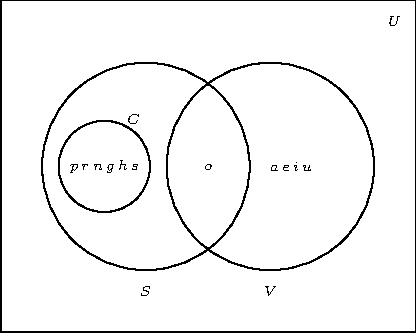
\includegraphics{SetTheory-1}

A Venn Diagram for $C$, $S$ and $V$.  

\end{center}

In the Venn Diagram above we have three circles - one for each of the sets $C$, $S$ and $V$.  We visualize the area enclosed by each of these circles as the elements of each set.  Here, we've spelled out the elements for definitiveness.  Notice that the circle representing the set $C$ is completely inside the circle representing $S$.  This is a geometric way of  showing that $C \subseteq S$.  Also, notice that the circles representing $S$ and $V$ overlap on the letter `o'.  This common region is how we visualize $S \cap V$.  Notice that since $C \cap V = \emptyset$, the circles which represent $C$ and $V$ have no overlap whatsoever.   

\medskip

All of these circles lie in a rectangle labeled $U$ (for `universal' set).  A universal set contains all of the elements under discussion, so it could always be taken as the union of all of the sets in question, or an even larger set.  In this case, we could take $U = S \cup V$ or $U$ as the set of letters in the entire alphabet.  The reader may well wonder if there is an ultimate universal set which contains \textit{everything}.  The short answer is `no' and we refer you once again to \href{http://en.wikipedia.org/wiki/Russell's_paradox}{\underline{Russell's Paradox}}.  The usual triptych of Venn Diagrams indicating generic sets $A$ and  $B$ along with $A \cap B$ and $A \cup B$ is given below.

\begin{center}

\begin{tabular}{ccc}


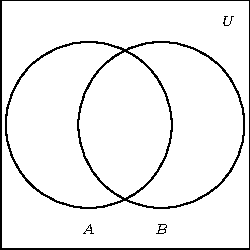
\includegraphics{SetTheory-2}



&

\hspace{0.15in}

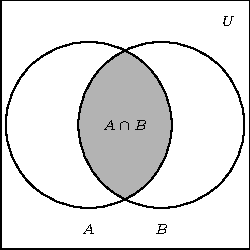
\includegraphics{SetTheory-3}

&

\hspace{0.15in}

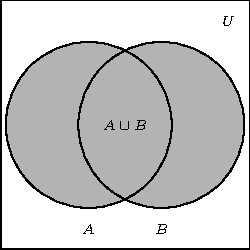
\includegraphics{SetTheory-4}

\\

Sets $A$ and $B$. 



&

\hspace{0.15in}

$A \cap B$ is shaded.

&

\hspace{0.15in}

$A \cup B$ is shaded.

\\
\end{tabular}

\end{center}

\section{Sets of Real Numbers}
\label{SetsofRealNumbers}

The playground for most of this text is the set of \textbf{Real Numbers}.  Many quantities in the `real world' can be quantified using real numbers: the temperature at a given time, the revenue generated by selling a certain number of products and the maximum population of Sasquatch which can inhabit a particular region are just three basic examples.   A succinct, but nonetheless incomplete\footnote{Math pun intended!} definition of a real number is given below.

\medskip

\colorbox{ResultColor}{\bbm

\begin{defn} \label{realnumberdefn}

A \textbf{real number}\index{real number ! set of}\index{real number ! definition of} is any number which possesses a decimal representation.  The set of real numbers is denoted by the character $\mathbb{R}$.  

\end{defn}

\ebm}

\medskip

Certain subsets of the real numbers are worthy of note and are listed below.  In fact, in more advanced texts,\footnote{See, for instance, Landau's \underline{Foundations of Analysis}.}   the real numbers are \textit{constructed} from some of these subsets.  

\medskip

\phantomsection
\label{setsofnumbersboxonthispage}

\colorbox{ResultColor}{\bbm

\centerline{\textbf{Special Subsets of Real Numbers}}\index{set ! sets of real numbers}

\begin{enumerate}

\item The \textbf{Natural Numbers}:\index{natural number ! set of}\index{natural number ! definition of} $\mathbb{N}= \{ 1, 2, 3,  \ldots\}$ The periods of ellipsis `$\ldots$' here indicate that the natural numbers contain $1$, $2$, $3$ `and so forth'.

%\item The \textbf{Whole Numbers}:\index{whole number ! set of}\index{whole number ! definition of} $\W = \{ 0, 1, 2, \ldots \}.$

\item The \textbf{Integers}:\index{integer ! set of}\index{integer ! definition of} $\mathbb Z=\{ \ldots, -3, -2, -1, 0, 1, 2, 3, \ldots \} = \{ 0, \pm 1, \pm 2, \pm 3, \ldots\}.$\footnote{The symbol $\pm$ is read `plus or minus' and it is a shorthand notation which appears throughout the text.  Just remember that $x = \pm 3$ means $x = 3$ or $x = -3$.}

\item The \textbf{Rational Numbers}:\index{rational number ! set of}\index{rational number ! definition of} $\mathbb{Q}=\left\{\frac{a}{b} \, | \, a \in \mathbb Z \, \mbox{and} \, b \in \mathbb Z \right\}$.  \underline{Ratio}nal numbers are the \underline{ratio}s of integers where the denominator is not zero.  It turns out that another way to describe the rational numbers is: \[\mathbb{Q}=\{x\,|\,\mbox{$x$ possesses a repeating or terminating decimal representation}\}\]

\item The \textbf{Irrational Numbers}:\index{irrational number ! set of}\index{irrational number ! definition of} The irrational numbers are those real numbers that are not rational. As a set, we have  $\{x\in\mathbb{R}\,|\,x\notin\mathbb{Q}\}$.\footnote{Examples here include number $\pi$, $\sqrt{2}$ and $0.101001000100001\ldots$. Note that there is no standard notation for the set of irrational numbers.}  In terms of decimal representation, the irrational numbers are those whose decimal expansion neither repeats nor terminates.

\end{enumerate}

\ebm}

\medskip

Note that every natural number is a whole number which, in turn, is an integer.   Each integer is a rational number (take $b =1$ in the above definition for $\mathbb{Q}$) and since every rational number is a real number\footnote{Thanks to long division!}  the sets $\mathbb{N}$,   $\mathbb Z$, $\mathbb{Q}$, and  $\mathbb{R}$ are nested like \href{http://en.wikipedia.org/wiki/Matryoshka_doll}{\underline{Matryoshka dolls}}. More formally, these sets form a subset chain:  $\mathbb{N} \subseteq \mathbb Z \subseteq \mathbb{Q} \subseteq \mathbb{R}$.  The reader is encouraged to sketch a Venn Diagram depicting $\mathbb{R}$ and all of the subsets mentioned above.  It is time for an example.

\begin{ex} \label{numbersetex}   $~$

\begin{enumerate}

\item  Write a roster description for $P = \{ 2^{n} \, | \, n \in \mathbb{N} \}$  and $E = \{ 2n \, | \, n \in \mathbb Z \}$.

\item Write a verbal description for $S = \{ x^2 \, | \, x \in \mathbb{R} \}$.

\item Let $A = \{-117, \frac{4}{5}, 0.20\overline{2002}, 0.202002000200002 \ldots\}$. 
Which elements of $A$ are natural numbers?  Rational numbers?  Real numbers?

\item  What is another name for $\mathbb{N} \cup \mathbb{Q}$?  What about  $\mathbb{Q} \cup \mathbb P$, where (for this example) we let $\mathbb{P}$ denote the set of irrational numbers?

\end{enumerate}

{\bf Solution.}

\begin{enumerate}

\item  To find a roster description for these sets, we need to list their elements.   Starting with $P = \{ 2^{n} \, | \, n \in \mathbb{N} \}$, we substitute natural number values $n$ into the formula $2^n$.  For $n = 1$ we get $2^1 = 2$,  for $n = 2$ we get $2^2 = 4$, for $n = 3$ we get $2^3 = 8$ and for $n = 4$ we get $2^4 = 16$.  Hence  $P$ describes the powers of $2$, so a roster description for $P$ is $P = \{ 2, 4, 8, 16, \ldots \}$ where the `$\ldots$' indicates the that pattern continues.\footnote{This isn't the most \textit{precise} way to describe this set - it's always dangerous to use `$\ldots$' since we assume that the pattern is clearly demonstrated and thus made evident to the reader.  Formulas are more precise because the pattern is clear.}  

\smallskip

Proceeding in the same way, we generate elements in $E = \{ 2n \, | \, n \in \mathbb Z \}$ by plugging in integer values of $n$ into the formula $2n$.  Starting with $n = 0$ we obtain $2(0) = 0$.  For $n = 1$ we get $2(1) = 2$, for $n = -1$ we get $2(-1) = -2$ for $n = 2$, we get $2(2) = 4$ and for $n = -2$ we get $2(-2) = -4$.  As $n$  moves through the integers, $2n$ produces all of the \textit{even} integers.\footnote{This shouldn't be too surprising, since an even integer is \textit{defined} to be an integer multiple of $2$.} A roster description for  $E$ is $E = \{ 0, \pm 2, \pm 4, \ldots \}$.

\item  One way to verbally describe $S$ is to say that $S$ is the `set of all squares of real numbers'.  While this isn't incorrect, we'd like to take this opportunity to delve a little deeper.\footnote{Think of this as an opportunity to stop and smell the mathematical roses.}  What makes the set $S = \{ x^2 \, | \, x \in \mathbb{R} \}$ a little trickier to wrangle than the sets $P$ or $E$ above is that the dummy variable here, $x$, runs through all \textit{real} numbers.  Unlike the natural numbers or the integers, the real numbers cannot be listed in any methodical way.\footnote{This is a nontrivial statement.  Interested readers are directed to a discussion of \href{http://en.wikipedia.org/wiki/Cantor's_diagonal_argument}{\underline{Cantor's Diagonal Argument}}.}  Nevertheless, we can select some real numbers, square them and get a sense of what kind of numbers lie in $S$.  For $x = -2$, $x^2 = (-2)^2 = 4$ so $4$ is in $S$, as are $\left(\frac{3}{2}\right)^2 = \frac{9}{4}$ and $(\sqrt{117})^2 = 117$.  Even things like $(-\pi)^2$ and $(0.101001000100001 \ldots)^2$ are in $S$.  

\smallskip

So suppose $s \in S$.  What can be said about $s$?  We know there is some real number $x$ so that $s = x^2$.  Since $x^2 \geq 0$ for any real number $x$, we know $s \geq 0$.  This tells us that everything in $S$ is a non-negative real number.\footnote{This means $S$ is a subset of the non-negative real numbers.}  This begs the question:  are \underline{all} of the non-negative real numbers in $S$?  Suppose $n$ is a non-negative real number, that is, $n \geq 0$.  If $n$ were in $S$, there would be a real number $x$ so that $x^2=n$.  As you may recall, we can solve $x^2 = n$ by `extracting square roots':  $x = \pm \sqrt{n}$.  Since $n \geq 0$, $\sqrt{n}$ is a real number.\footnote{This is called the `square root closed' property of the non-negative real numbers.}  Moreover, $(\sqrt{n})^2 = n$ so $n$ is the square of a real number which means $n \in S$. Hence, $S$ is the set of non-negative real numbers.

\item   The set $A$ contains no natural numbers.\footnote{Carl was tempted to include $0.\overline{9}$ in the set $A$, but thought better of it.  }  Clearly, $\frac{4}{5}$ is a rational number as is $-117$ (which can be written as $\frac{-117}{1}$). It's the last two numbers listed in $A$, $0.20\overline{2002}$ and $0.202002000200002 \ldots$, that warrant some discussion.  First, recall that the `line' over the digits $2002$ in $0.20\overline{2002}$ (called the vinculum) indicates that these digits repeat, so it is a rational number.\footnote{So $0.20\overline{2002} = 0.20200220022002 \ldots$.}  As for the number $0.202002000200002 \ldots$, the `$\ldots$' indicates the pattern of adding an extra `$0$' followed by a `$2$' is what defines this real number.  Despite the fact there is a \textit{pattern} to this decimal, this decimal is \textit{not repeating}, so it is not a rational number - it is, in fact, an irrational number.  All of the elements of $A$ are real numbers, since all of them can be expressed as decimals (remember that $\frac{4}{5} = 0.8$).

%\item  The set $A \cap \W = \{ x \, | \, \text{$x \in A$ and $x \in \W$} \}$ is another way of saying we are looking for the set of numbers in $A$ which are whole numbers.  Since $A$ contains no whole numbers, $A \cap \W = \emptyset$.  Similarly, $A \cap \mathbb Z$ is looking for the set of numbers in $A$ which are integers.  Since $-117$ is the only integer in $A$,  $A \cap \mathbb Z = \{ -117 \}$. As for the set $A \cap \mathbb P$, as discussed in part (a), the number $0.202002000200002 \ldots$ is irrational, so $A \cap \mathbb P = \{ 0.202002000200002 \ldots \}$.


\item  The set $\mathbb{N} \cup \mathbb{Q} = \{ x \, | \, \text{$x \in \mathbb{N}$ or $x \in \mathbb{Q}$} \}$ is the union of the set of natural numbers with the set of rational numbers.  Since every natural number is a rational number, $\mathbb{N}$ doesn't contribute any new elements to $\mathbb{Q}$, so $\mathbb{N} \cup \mathbb{Q} = \mathbb{Q}$.\footnote{In fact, any time $A \subseteq B$, $A \cup B = B$ and vice-versa.  See the exercises.}  For the  set $\mathbb{Q} \cup \mathbb P$, we note that every real number is either rational or not, hence $\mathbb{Q} \cup \mathbb P = \mathbb{R}$, pretty much by the definition of the set $\mathbb P$.  \qed


\end{enumerate}


\end{ex}

As you may recall, we often visualize the set of real numbers $\mathbb{R}$ as a line where each point on the line corresponds to one and only one real number.  Given two different real numbers $a$ and $b$,  we write $a < b$ if $a$ is located to the left of $b$ on the number line, as shown below.

\begin{center}

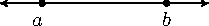
\includegraphics{SetTheory-5}

The real number line with two numbers $a$ and $b$ where $a < b$.

\end{center}

While this notion seems innocuous, it is worth pointing out that this convention is rooted in two deep properties of real numbers.  The first property is that $\mathbb{R}$ is  \href{http://en.wikipedia.org/wiki/Complete_metric_space}{\underline{complete}}. This means that there are no `holes' or `gaps' in the real number line.\footnote{Alas, this intuitive feel for what it means to be `complete' is as good as it gets at this level.  Completeness does get a much more precise meaning later in courses like Analysis and Topology.} Another way to think about this is that if you choose any two distinct (different) real numbers, and look between them, you'll find a solid line segment (or interval) consisting of infinitely many real numbers.  The next result tells us what types of numbers we can expect to find.

\medskip

\phantomsection
\label{densityofqandp}

\colorbox{ResultColor}{\bbm

\centerline{\textbf{Density Property of $\mathbb{Q}$ in $\mathbb{R}$}}

Between any two distinct real numbers, there is at least one rational number and irrational number.  It then follows that between any two distinct real numbers there will be \underline{infinitely many} rational and irrational numbers.

\ebm}

\medskip

The root word `dense' here communicates the idea that rationals and irrationals are `thoroughly mixed' into $\mathbb{R}$.   The reader is encouraged to think about how one would find both a rational and an irrational number between, say, $0.9999$ and $1$. Once you've done that, try doing the same thing for the numbers $0.\overline{9}$ and $1$. (`Try' is the operative word, here.

\smallskip

The second property $\mathbb{R}$ possesses that lets us view it as a line is that the set is \href{http://en.wikipedia.org/wiki/Total_order}{\underline{totally ordered}}. This means that given any two real numbers $a$ and $b$, either $a < b$, $a > b$ or $a = b$ which allows us to arrange the numbers from least (left) to greatest (right). You may have heard this property given as the `Law of Trichotomy'.\index{trichotomy}

\medskip

\phantomsection
\label{trichotomy}

\colorbox{ResultColor}{\bbm

\centerline{\textbf{Law of Trichotomy}}

If $a$ and $b$ are real numbers then exactly one of the following statements is true: \vspace{-.15in} \[ \begin{array}{lclcl} a < b & \hspace*{1.25in} & a > b & \hspace*{1.25in} & a = b \end{array} \]

\ebm}

\medskip

Segments of the real number line are called \textbf{intervals}.\index{interval ! definition of}  They play a huge role not only in this text but also in the Calculus curriculum so we need a concise way to describe them.  We start by examining a few examples of the \textbf{interval notation}\index{interval ! notation for} associated with some specific sets of numbers.  

\begin{center}
\begin{tabular}{|c|c|c|} \hline

Set of Real Numbers & Interval Notation &  Region on the Real Number Line  \\
\hline

& &  \\
\shortstack{$\{x\,|\,1\leq x< 3\}$ \\ \hfill} & \shortstack{$[1,3)$ \\ \hfill} & 

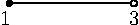
\includegraphics{SetTheory-6}   \\
\hline

 &  & \\
\shortstack{$\{x\,|\,-1\leq x \leq 4\}$ \\ \hfill}& \shortstack{$[-1,4]$ \\ \hfill} & 

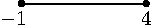
\includegraphics{SetTheory-7}   \\
\hline

&  & \\

\shortstack{$\{x\,| \, x \leq 5 \}$ \\ \hfill} & \shortstack{$(-\infty, 5]$ \\ \hfill} &

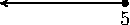
\includegraphics{SetTheory-8}   \\
\hline

 &  & \\
\shortstack{$\{x\,| \, x > -2 \}$ \\ \hfill} & \shortstack{$(-2, \infty)$ \\ \hfill} &  

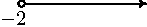
\includegraphics{SetTheory-9}   \\
\hline

\end{tabular}

\end{center}

As you can glean from the table, for intervals with finite endpoints we start by writing `left endpoint, right endpoint'.  We use square brackets, `$[$' or `$]$', if the endpoint is included in the interval. This corresponds to a `filled-in' or `closed' dot on the number line to indicate that the number is included in the set.  Otherwise, we use parentheses, `$($' or `$)$' that correspond to an `open' circle which indicates that the endpoint is not part of the set.  If the interval does not have finite endpoints, we use the symbol $-\infty$ to indicate that the interval extends indefinitely to the left and the symbol $\infty$ to indicate that the interval extends indefinitely to the right.  Since infinity is a concept, and not a number, we always use parentheses when using these symbols in interval notation, and use the appropriate arrow to indicate that the interval extends indefinitely in one or both directions. We summarize all of the possible cases in one convenient table below.\footnote{The importance of understanding interval notation in Calculus cannot be overstated so please do yourself a favor and memorize this chart.}

\medskip

\phantomsection
\label{intervalnotationsummary}

\colorbox{ResultColor}{\bbm

%\smallskip

\centerline{\textbf{Interval Notation}}

\medskip

\hspace{.5in} Let $a$ and $b$ be real numbers with $a<b$.

\smallskip

\begin{center}

\begin{tabular}{|c|c|c|} \hline

Set of Real Numbers & Interval Notation &  Region on the Real Number Line  \\
\hline

 &  & \\
\shortstack{$\{x\,|\,a<x<b\}$ \\ \hfill}& \shortstack{$(a,b)$ \\ \hfill} & 

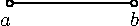
\includegraphics{SetTheory-10}  \\ \hline

& &  \\
\shortstack{$\{x\,|\,a\leq x<b\}$ \\ \hfill}& \shortstack{$[a,b)$ \\ \hfill} & 

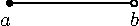
\includegraphics{SetTheory-11}   \\
\hline

 &  & \\
\shortstack{$\{x\,|\,a<x\leq b\}$ \\ \hfill}&\shortstack{$(a,b]$ \\ \hfill} & 

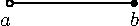
\includegraphics{SetTheory-12}   \\
\hline

 &  & \\
\shortstack{$\{x\,|\,a\leq x \leq b\}$ \\ \hfill}& \shortstack{$[a,b]$ \\ \hfill}& 

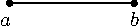
\includegraphics{SetTheory-13}   \\
\hline

 & & \\
\shortstack{$\{x\,| \, x<b\}$ \\ \hfill}& \shortstack{$(-\infty,b)$ \\ \hfill}& 

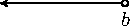
\includegraphics{SetTheory-14}   \\
\hline


&  & \\

\shortstack{$\{x\,| \, x \leq b\}$ \\ \hfill} & \shortstack{$(-\infty,b]$ \\ \hfill}& 

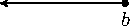
\includegraphics{SetTheory-15}   \\
\hline

 &  & \\
\shortstack{$\{x\,| \, x>a\}$ \\ \hfill}& \shortstack{$(a,\infty)$ \\ \hfill}& 

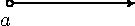
\includegraphics{SetTheory-16}   \\
\hline

 &  & \\
\shortstack{$\{x\,| \, x \geq a \}$ \\ \hfill}& \shortstack{$[a,\infty)$ \\ \hfill} & 

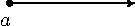
\includegraphics{SetTheory-17}   \\
\hline

&  & \\
\shortstack{$\mathbb{R}$ \\ \hfill}& \shortstack{$(-\infty,\infty)$ \\ \hfill} & 

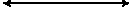
\includegraphics{SetTheory-18}   \\
\hline

\end{tabular}

\end{center}

\ebm}

\medskip

We close this section with an example that ties together several concepts presented earlier.  Specifically, we demonstrate how to use interval notation along with the concepts of `union' and `intersection' to describe a variety of sets on the real number line.

\begin{ex} \label{intervalex} $~$

\begin{enumerate} \item Express the following sets of numbers using interval notation.

\begin{multicols}{2}

\begin{enumerate}

\item  $\{ x \, | \, x \leq -2 \, \, \text{or} \, \,  x \geq 2 \}$

\item  $\{ x \, | \, x \neq 3 \}$

\setcounter{HW}{\value{enumii}}

\end{enumerate}

\end{multicols}

\begin{multicols}{2}

\begin{enumerate}

\setcounter{enumii}{\value{HW}}

\item  $\{ x \, | \, x \neq \pm 3 \}$

\item  $\{ x \, | \, -1 < x \leq 3 \,\, \text{or} \,\, x = 5\}$

\end{enumerate}

\end{multicols}

\item  Let $A = [-5,3)$ and $B = (1, \infty)$.  Find  $A \cap B$ and $A\cup B$. 

\end{enumerate}


{\bf Solution.}

\begin{enumerate}

\item 

\begin{enumerate}

\item  The best way to proceed here is to graph the set of numbers on the number line and glean the answer from it.  The inequality $x \leq -2$ corresponds to the interval $(-\infty, -2]$ and the inequality $x \geq 2$ corresponds to the interval $[2, \infty)$. The `or' in $\{ x \, | \, x \leq -2 \, \, \text{or} \, \,  x \geq 2 \}$ tells us that we are looking for the union of these two intervals, so our answer is $(-\infty, -2] \cup [2, \infty)$.

\begin{center}

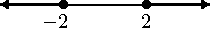
\includegraphics{SetTheory-19}  \\
$(-\infty, -2] \cup [2, \infty)$ 

\end{center}

\item For the set $\{ x \, | \, x \neq 3 \}$, we shade the entire real number line except $x=3$, where we leave an open circle.  This divides the real number line into two intervals, $(-\infty, 3)$ and $(3,\infty)$.  Since the values of $x$ could be in one of these intervals \textit{or} the other, we once again use the union symbol to get $\{ x \, | \, x \neq 3 \} = (-\infty, 3) \cup (3,\infty)$.
 
\begin{center}

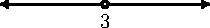
\includegraphics{SetTheory-20}  \\



 $(-\infty, 3) \cup (3, \infty)$ 
 
 

\end{center}

\item  For the set $\{ x \, | \, x \neq \pm 3 \}$, we proceed as before and exclude both $x=3$ and $x=-3$ from our set. (Do you remember what we said back on \pageref{setsofnumbersboxonthispage} about $x = \pm 3$?)  This breaks the number line into \textit{three} intervals, $(-\infty, -3)$, $(-3,3)$ and $(3, \infty)$.   Since the set describes real numbers which come from the first, second \textit{or} third interval, we have $\{ x \, | \, x \neq \pm 3 \} = (-\infty, -3) \cup (-3,3) \cup (3, \infty)$.


\begin{center}

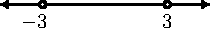
\includegraphics{SetTheory-21} \\

 $(-\infty, -3) \cup (-3,3) \cup (3, \infty)$
 
 \end{center}



\item  Graphing the set $\{ x \, | \, -1 < x \leq 3 \,\, \text{or} \,\, x = 5\}$ yields the interval $(-1,3]$ along with the single number 5.  While we \textit{could} express this single point as $[5,5]$, it is customary to write a single point as a `singleton set', so in our case we have the set $\{ 5\}$. Thus our final answer is $\{ x \, | \, -1 < x \leq 3 \,\, \text{or} \,\, x = 5\} = (-1,3] \cup \{ 5\}$.


\begin{center}

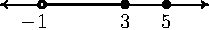
\includegraphics{SetTheory-22} \\
  
 $(-1,3] \cup \{ 5\}$
 
\end{center}


\end{enumerate}

\item  We start by graphing $A = [-5,3)$ and $B = (1, \infty)$ on the number line.  To find $A\cap B$, we need to find the numbers in common to both $A$ and $B$, in other words, the overlap of the two intervals.  Clearly, everything between $1$ and $3$ is in both $A$ and $B$.  However, since $1$ is in $A$ but not in $B$, $1$ is not in the intersection.  Similarly, since $3$ is in $B$ but not in $A$, it isn't in the intersection either.  Hence, $A \cap B = (1,3)$.  To find $A \cup B$, we need to find the numbers in at least one of $A$ or $B$.  Graphically, we shade $A$ and $B$ along with it.   Notice here that even though $1$ isn't in $B$, it is in $A$, so it's the union along with all the other elements of $A$ between $-5$ and $1$.  A similar argument goes for the inclusion of $3$ in the union.  The result of shading both $A$ and $B$ together gives us $A \cup B = [-5,\infty)$.

\begin{center}

\begin{tabular}{ccc}

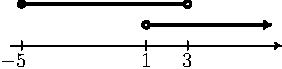
\includegraphics{SetTheory-23}  &

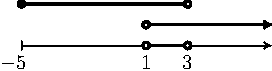
\includegraphics{SetTheory-24}  &

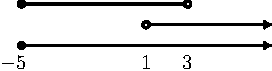
\includegraphics{SetTheory-25} \\

\end{tabular}

\end{center}

\end{enumerate}

\vspace*{-.4in} \qed

\end{ex}

\newpage

\section{Exercises}

\begin{enumerate}


\item  Find a verbal description for $O = \{ 2n-1 \, | \, n \in \mathbb{N}\}$


\item  Find a roster description for $X = \{ z^2 \, | \, z \in \mathbb{Z}\}$


\item  Let $A = \left\{ -3, -1.02, -\dfrac{3}{5}, 0.57, 1.\overline{23}, \sqrt{3}, 5.2020020002 \ldots, \dfrac{20}{10}, 117 \right\}$ 

\begin{enumerate}

\item  List the elements of $A$ which are natural numbers.
\item  List the elements of $A$ which are irrational numbers.
\item  Find $A \cap \mathbb{Z}$
\item  Find $A \cap \mathbb{Q}$


\end{enumerate}


\item Fill in the chart below. 

\begin{center}
\begin{tabular}{|c|c|c|} \hline

Set of Real Numbers & Interval Notation &  Region on the Real Number Line  \\
\hline

& &  \\

\shortstack{$\{x\,|\,-1\leq x< 5\}$ \\ \hfill} &  &  \\ \hline

& &  \\

 & \shortstack{$[0,3)$ \\ \hfill} &   \\ \hline


& &  \\

 &  & 

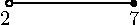
\includegraphics{SetTheory-26}   \\
\hline

 &  & \\
 
\shortstack{$\{x\,|\, -5 <  x \leq 0 \}$ \\ \hfill} &  & \\ \hline

 &  & \\
 
  & \shortstack{$(-3,3)$ \\ \hfill} &  \\ \hline

&  & \\
 
& & 

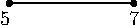
\includegraphics{SetTheory-27}   \\
\hline

&  & \\

\shortstack{$\{x\,| \, x \leq 3 \}$ \\ \hfill} &  &  \\ \hline

 &  & \\
 
& \shortstack{$(-\infty, 9)$ \\ \hfill} &  \\ \hline

 &  & \\

 &  &  

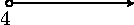
\includegraphics{SetTheory-28}   \\
\hline

 &  & \\
 
 
\shortstack{$\{x\,| \, x \geq  -3 \}$ \\ \hfill} & &    \\ \hline

\end{tabular}

\end{center}

\setcounter{HW}{\value{enumi}}
\end{enumerate}

\newpage

In Exercises \ref{findunionintfirst} - \ref{findunionintlast}, find the indicated intersection or union and simplify if possible.  Express your answers in interval notation. 

\begin{multicols}{3}
\begin{enumerate}
\setcounter{enumi}{\value{HW}}

\item  $(-1,5] \cap [0,8)$ \label{findunionintfirst}
\item  $(-1,1) \cup [0,6]$
\item $(-\infty,4]\cap (0,\infty)$

\setcounter{HW}{\value{enumi}}
\end{enumerate}
\end{multicols}

\begin{multicols}{3}
\begin{enumerate}
\setcounter{enumi}{\value{HW}}

\item $(-\infty,0) \cap [1,5]$
\item $(-\infty, 0) \cup [1,5]$
\item $(-\infty, 5] \cap [5,8)$ \label{findunionintlast}

\setcounter{HW}{\value{enumi}}
\end{enumerate}
\end{multicols}

In Exercises \ref{writeintervalfirst} - \ref{writeintervallast}, write the set using interval notation.   

\begin{multicols}{3}
\begin{enumerate}
\setcounter{enumi}{\value{HW}}

\item  $\{x\,|\, x \neq 5 \}$ \label{writeintervalfirst}
\item  $\{x\,|\, x \neq -1 \}$
\item  $\{x\,|\, x \neq -3,\, 4 \}$

\setcounter{HW}{\value{enumi}}
\end{enumerate}
\end{multicols}

\begin{multicols}{3}
\begin{enumerate}
\setcounter{enumi}{\value{HW}}

\item  $\{x\,|\, x \neq 0, \, 2 \}$
\item  $\{x\,|\, x \neq 2, \, -2 \}$
\item  $\{x\,|\, x \neq 0,\, \pm 4 \}$

\setcounter{HW}{\value{enumi}}
\end{enumerate}
\end{multicols}

\begin{multicols}{3}
\begin{enumerate}
\setcounter{enumi}{\value{HW}}

\item $\{x\,|\, x \leq -1 \, \text{or} \, x \geq 1 \}$
\item $\{x\,|\, x < 3 \, \text{or} \, x \geq 2 \}$
\item $\{x\,|\, x \leq -3 \, \text{or} \, x > 0 \}$

\setcounter{HW}{\value{enumi}}
\end{enumerate}
\end{multicols}

\begin{multicols}{3}
\begin{enumerate}
\setcounter{enumi}{\value{HW}}

\item $\{x\,|\, x \leq 5 \, \text{or} \, x = 6 \}$
\item $\{x\,|\, x > 2 \, \text{or} \, x = \pm 1 \}$
\item $\{x\,|\,  -3 < x < 3 \, \text{or} \, x = 4 \}$ \label{writeintervallast}

\setcounter{HW}{\value{enumi}}
\end{enumerate}
\end{multicols}

For Exercises \ref{shadevennfirst} - \ref{shadevennlast}, use the blank Venn Diagram below $A$, $B$, and $C$ as a guide for you to shade the following sets.

\begin{center}
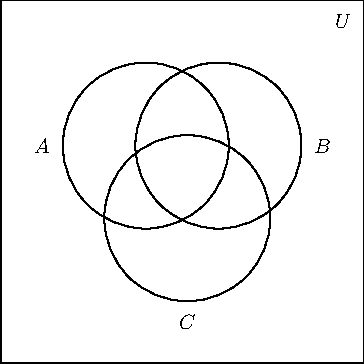
\includegraphics{SetTheory-29}

\end{center}

\begin{multicols}{3}
\begin{enumerate}
\setcounter{enumi}{\value{HW}}

\item  $A \cup C$ \label{shadevennfirst}

\item  $B \cap C$

\item  $(A \cup B) \cup C$



\setcounter{HW}{\value{enumi}}
\end{enumerate}
\end{multicols}

\begin{multicols}{3}
\begin{enumerate}
\setcounter{enumi}{\value{HW}}

\item  $(A \cap B) \cap C$ 

\item  $A \cap (B \cup C)$ \label{intoverunion}

\item  $(A \cap B) \cup (A \cap C)$ \label{shadevennlast}

\setcounter{HW}{\value{enumi}}
\end{enumerate}
\end{multicols}

\begin{enumerate}
\setcounter{enumi}{\value{HW}}

\item  Explain how your answers to problems \ref{intoverunion} and \ref{shadevennlast} show $A \cap (B \cup C) = (A \cap B) \cup (A \cap C)$.  Phrased differently, this shows `intersection \textit{distributes} over union.'  Discuss with your classmates if  `union' distributes over `intersection.'  Use a Venn Diagram to support your answer.

\setcounter{HW}{\value{enumi}}
\end{enumerate}

\newpage

\section{Answers}

\begin{enumerate}


\item  $O$ is the odd natural numbers.


\item  $X = \{ 0, 1, 4, 9, 16, \ldots \}$


\item  \begin{enumerate} \item  $\dfrac{20}{10} = 2$ and $117$
\item  $\sqrt{3}$ and $5.2020020002$
\item $\left\{ -3, \dfrac{20}{10}, 117\right\}$
\item  $\left\{ -3, -1.02, -\dfrac{3}{5}, 0.57, 1.\overline{23},\dfrac{20}{10}, 117 \right \}$

\end{enumerate}

\item $~$

\begin{center}
\begin{tabular}{|c|c|c|} \hline

Set of Real Numbers & Interval Notation &  Region on the Real Number Line  \\
\hline

& &  \\

\shortstack{$\{x\,|\,-1\leq x< 5\}$ \\ \hfill} & \shortstack{$[-1,5)$ \\ \hfill} & 

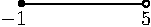
\includegraphics{SetTheory-30}   \\
\hline

& &  \\

\shortstack{$\{x\,|\,0\leq x < 3\}$ \\ \hfill} & \shortstack{$[0,3)$ \\ \hfill} & 

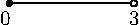
\includegraphics{SetTheory-31}   \\
\hline


& &  \\

\shortstack{$\{x\,|\, 2 <  x \leq 7 \}$ \\ \hfill} & \shortstack{$(2,7]$ \\ \hfill} & 

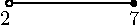
\includegraphics{SetTheory-32}   \\
\hline

 &  & \\
 
 \shortstack{$\{x\,|\, -5 <  x \leq 0 \}$ \\ \hfill} & \shortstack{$(-5,0]$ \\ \hfill} & 

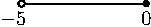
\includegraphics{SetTheory-33}   \\
\hline

 &  & \\
 
 \shortstack{$\{x\,|\, -3 <  x < 3 \}$ \\ \hfill} & \shortstack{$(-3,3)$ \\ \hfill} & 

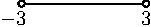
\includegraphics{SetTheory-34}   \\
\hline

 &  & \\
 
\shortstack{$\{x\,|\,5\leq x \leq 7\}$ \\ \hfill}& \shortstack{$[5,7]$ \\ \hfill} & 

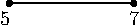
\includegraphics{SetTheory-35}   \\
\hline

&  & \\

\shortstack{$\{x\,| \, x \leq 3 \}$ \\ \hfill} & \shortstack{$(-\infty, 3]$ \\ \hfill} &
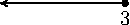
\includegraphics{SetTheory-36}   \\
\hline

 &  & \\
 
 \shortstack{$\{x\,| \, x < 9 \}$ \\ \hfill} & \shortstack{$(-\infty, 9)$ \\ \hfill} &
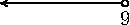
\includegraphics{SetTheory-37}   \\
\hline

 &  & \\
 
 
\shortstack{$\{x\,| \, x >  4 \}$ \\ \hfill} & \shortstack{$(4, \infty)$ \\ \hfill} &  

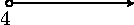
\includegraphics{SetTheory-38}   \\
\hline

 &  & \\
 
 
\shortstack{$\{x\,| \, x \geq  -3 \}$ \\ \hfill} & \shortstack{$[-3, \infty)$ \\ \hfill} &  

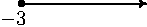
\includegraphics{SetTheory-39}   \\
\hline

\end{tabular}

\end{center}

\setcounter{HW}{\value{enumi}}
\end{enumerate}

\begin{multicols}{2}
\begin{enumerate}
\setcounter{enumi}{\value{HW}}

\item  $(-1,5] \cap [0,8) = [0,5]$

\item  $(-1,1) \cup [0,6] = (-1,6]$

\setcounter{HW}{\value{enumi}}
\end{enumerate}
\end{multicols}

\begin{multicols}{2}
\begin{enumerate}
\setcounter{enumi}{\value{HW}}

\item $(-\infty,4]\cap (0,\infty) = (0,4]$


\item $(-\infty,0) \cap [1,5] = \emptyset$

\setcounter{HW}{\value{enumi}}
\end{enumerate}
\end{multicols}

\begin{multicols}{2}
\begin{enumerate}
\setcounter{enumi}{\value{HW}}

\item $(-\infty, 0) \cup [1,5] = (-\infty,0) \cup [1,5]$

\item $(-\infty, 5] \cap [5,8) = \left\{ 5\right\}$

\setcounter{HW}{\value{enumi}}
\end{enumerate}
\end{multicols}

\begin{multicols}{2}
\begin{enumerate}
\setcounter{enumi}{\value{HW}}

\item  $(-\infty, 5) \cup (5, \infty)$

\item  $(-\infty, -1) \cup (-1, \infty)$

\setcounter{HW}{\value{enumi}}
\end{enumerate}
\end{multicols}


\begin{multicols}{2}
\begin{enumerate}
\setcounter{enumi}{\value{HW}}

\item  $(-\infty, -3) \cup (-3, 4)\cup (4, \infty)$


\item   $(-\infty, 0) \cup (0, 2)\cup (2, \infty)$

\setcounter{HW}{\value{enumi}}
\end{enumerate}
\end{multicols}


\begin{multicols}{2}
\begin{enumerate}
\setcounter{enumi}{\value{HW}}

\item  $(-\infty, -2) \cup (-2, 2)\cup (2, \infty)$

\item  $(-\infty, -4) \cup (-4, 0) \cup (0, 4) \cup (4, \infty)$

\setcounter{HW}{\value{enumi}}
\end{enumerate}
\end{multicols}

\begin{multicols}{2}
\begin{enumerate}
\setcounter{enumi}{\value{HW}}

\item $(-\infty, -1] \cup [1, \infty)$

\item $(-\infty, \infty)$


\setcounter{HW}{\value{enumi}}
\end{enumerate}
\end{multicols}


\begin{multicols}{2}
\begin{enumerate}
\setcounter{enumi}{\value{HW}}

\item $(-\infty, -3] \cup (0, \infty)$

\item $(-\infty, 5] \cup \{6\}$

\setcounter{HW}{\value{enumi}}
\end{enumerate}
\end{multicols}

\begin{multicols}{2}
\begin{enumerate}
\setcounter{enumi}{\value{HW}}


\item $\{-1\} \cup \{1\} \cup (2, \infty)$

\item $(-3,3) \cup \{4\}$

\setcounter{HW}{\value{enumi}}
\end{enumerate}
\end{multicols}


\begin{multicols}{2}
\begin{enumerate}
\setcounter{enumi}{\value{HW}}

\item $A \cup C$

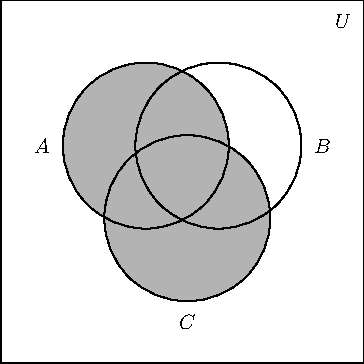
\includegraphics{SetTheory-40}

\item $B \cap C$

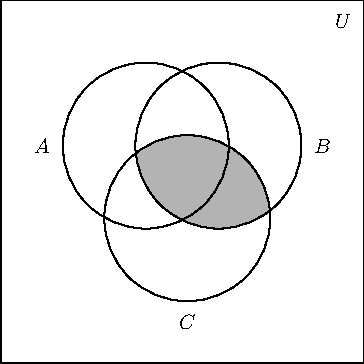
\includegraphics{SetTheory-41}



\setcounter{HW}{\value{enumi}}
\end{enumerate}
\end{multicols}

\pagebreak


\begin{multicols}{2}
\begin{enumerate}
\setcounter{enumi}{\value{HW}}


\item $(A \cup B) \cup C$

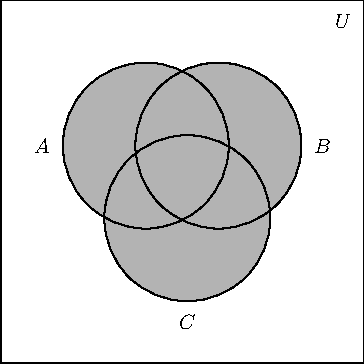
\includegraphics{SetTheory-42}


\item $(A \cap B) \cap C$

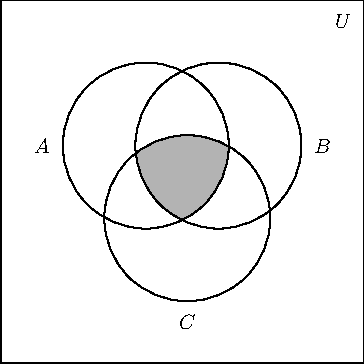
\includegraphics{SetTheory-43}



\setcounter{HW}{\value{enumi}}
\end{enumerate}
\end{multicols}

\begin{multicols}{2}
\begin{enumerate}
\setcounter{enumi}{\value{HW}}


\item $A \cap (B \cup C)$

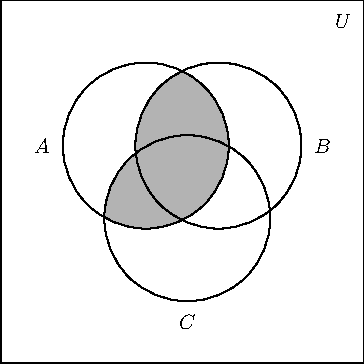
\includegraphics{SetTheory-44}


\item $(A \cap B) \cup (A \cap C)$ 

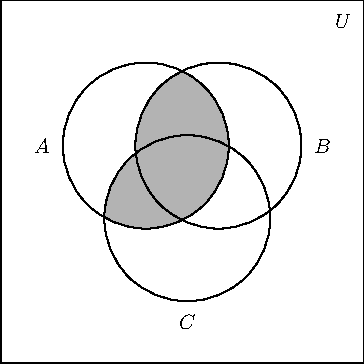
\includegraphics{SetTheory-45}




\setcounter{HW}{\value{enumi}}
\end{enumerate}
\end{multicols}
\enlargethispage{2in}

\begin{enumerate}
\setcounter{enumi}{\value{HW}}

\item  Yes, $A \cup (B \cap C) = (A \cup B) \cap (A \cup C)$.

\begin{center}

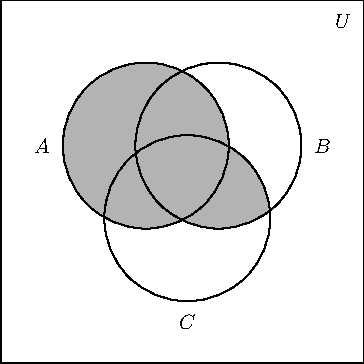
\includegraphics{SetTheory-46}


\end{center}

\setcounter{HW}{\value{enumi}}
\end{enumerate}

\end{document}